% Use only LaTeX2e, calling the article.cls class and 12-point type.

\documentclass[12pt]{article}

% Users of the {thebibliography} environment or BibTeX should use the
% scicite.sty package, downloadable from *Science* at
% http://www.sciencemag.org/authors/preparing-manuscripts-using-latex 
% This package should properly format in-text
% reference calls and reference-list numbers.

\usepackage{scicite}
\usepackage{graphicx}
\usepackage{times}

% The preamble here sets up a lot of new/revised commands and
% environments.  It's annoying, but please do *not* try to strip these
% out into a separate .sty file (which could lead to the loss of some
% information when we convert the file to other formats).  Instead, keep
% them in the preamble of your main LaTeX source file.


% The following parameters seem to provide a reasonable page setup.

\topmargin 0.0cm
\oddsidemargin 0.2cm
\textwidth 16cm 
\textheight 21cm
\footskip 1.0cm


%The next command sets up an environment for the abstract to your paper.

\newenvironment{sciabstract}{%
\begin{quote} \bf}
{\end{quote}}



% Include your paper's title here

\title{Basic Template for DML} 


% Place the author information here.  Please hand-code the contact
% information and notecalls; do *not* use \footnote commands.  Let the
% author contact information appear immediately below the author names
% as shown.  We would also prefer that you don't change the type-size
% settings shown here.

\author
{John Smith,$^{1\ast}$ Jane Doe,$^{1}$ Joe Scientist$^{2}$\\
\\
\normalsize{$^{1}$Department of Chemistry, University of Wherever,}\\
\normalsize{An Unknown Address, Wherever, ST 00000, USA}\\
\normalsize{$^{2}$Another Unknown Address, Palookaville, ST 99999, USA}\\
\\
\normalsize{$^\ast$To whom correspondence should be addressed; E-mail:  jsmith@wherever.edu.}
}

% Include the date command, but leave its argument blank.

\date{}



%%%%%%%%%%%%%%%%% END OF PREAMBLE %%%%%%%%%%%%%%%%



\begin{document} 

% Double-space the manuscript.

\baselineskip24pt

% Make the title.

\maketitle 



% Place your abstract within the special {sciabstract} environment.

\begin{sciabstract}
  This document presents a number of hints about how to set up your
  {\it Science\/} paper in \LaTeX\ .  We provide a template file,
  \texttt{scifile.tex}, that you can use to set up the \LaTeX\ source
  for your article.  An example of the style is the special
  \texttt{\{sciabstract\}} environment used to set up the abstract you
  see here.
\end{sciabstract}



% In setting up this template for *Science* papers, we've used both
% the \section* command and the \paragraph* command for topical
% divisions.  Which you use will of course depend on the type of paper
% you're writing.  Review Articles tend to have displayed headings, for
% which \section* is more appropriate; Research Articles, when they have
% formal topical divisions at all, tend to signal them with bold text
% that runs into the paragraph, for which \paragraph* is the right
% choice.  Either way, use the asterisk (*) modifier, as shown, to
% suppress numbering.

\section*{Start}

Initially, the problem at hand must be meticulously defined. What constitutes the input data? What are the desired outputs? What predictions are sought after? Furthermore, discerning the nature of the problem is crucial. Is it a classification task? Regression? Or does it entail a different paradigm altogether? Determining the appropriate architectural framework is equally pivotal.

Progression to subsequent stages hinges upon a comprehensive understanding of the inputs, outputs, and data sources. Without this clarity, advancement becomes untenable.

Quality assurance of the data is imperative, coupled with a profound comprehension of its characteristics. It's essential to acknowledge that even with meticulous definition of inputs, architecture, etc., certain challenges may persist, particularly in the realm of nonstationary problems. It's a stark reminder that recognition is restricted to previously encountered patterns.

Furthermore, it is imperative to establish the desired outputs and devise methodologies for their assessment to ascertain the efficacy of our model. Determining whether the model is functioning optimally necessitates a thorough evaluation strategy.

Various predefined metrics cater to specific problem domains. For balanced-classification quandaries, characterized by equiprobable classes, metrics such as accuracy and the area under the receiver operating characteristic curve (ROC AUC) are widely employed. Conversely, in scenarios marked by class imbalances, precision and recall serve as more pertinent measures. For tasks involving ranking or multilabel classification, mean average precision is a favored metric. Additionally, there are instances wherein the formulation of custom evaluation metrics becomes imperative.

With the evaluation framework in place, the subsequent phase involves data preparation and model input. In the realm of deep neural networks, which operate on tensors, data transformation into compact and heterogeneous values is essential. Concurrently, leveraging feature engineering techniques can augment model performance.

When delineating a model for a given problem, the primary objective invariably revolves around surpassing the performance of baseline statistical methods. Failing to outperform these benchmarks renders the model redundant, as basic statistical computations suffice for generating predictions.

Should initial attempts at model improvement fall short of surpassing the established baseline, several strategies can be explored:
\begin{itemize}
    \item Last-layer activation
    \item Loss function
    \item Optimization configuration
\end{itemize}
 In Figure 1 we have some help regarding those elections:
\begin{figure}
    \centering
    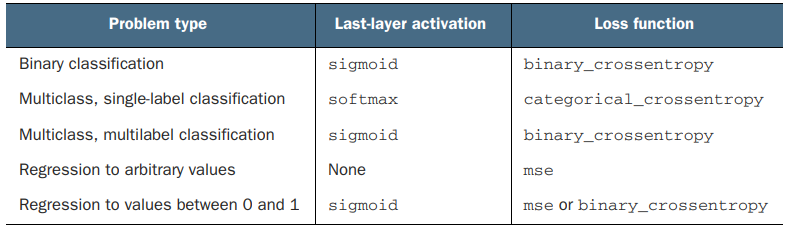
\includegraphics[width=1\linewidth]{image.png}
    \caption{Useful approaches}
    \label{fig:enter-label}
\end{figure}

Once the baseline has been obliterated, the critical question arises: when do we halt our pursuit? Is it when we achieve 100\% accuracy? Or perhaps when our model exhibits zero failures? The answer lies in navigating the perilous terrain of overfitting. It's a straightforward task; we discontinue when our model begins to exhibit signs of overfitting. However, this endeavor is deceptively simple to accomplish. One can simply augment the model's complexity by adding more layers, increasing their sizes, extending training epochs, or exploring various other avenues. Detection of overfitting can be conveniently gauged by monitoring the validation accuracy. When a decline is observed, it signals the onset of overfitting.

The subsequent phase involves refining our model until it achieves peak performance without succumbing to overfitting. Although this process entails a considerable investment of time and relies heavily on trial and error, it is nevertheless straightforward, but don't overdo it because you can overfit your validation data as well. One can experiment freely with a myriad of strategies aimed at enhancing the model's performance. Notable among these approaches include:
\begin{itemize}
    \item Add dropout
    \item Add/remove layers
    \item Use regularization
    \item Change the learning rate
    \item Change how you have represented your data/Feature engineering
\end{itemize}
\section*{}











\section*{What to Send In}

What you should send to {\it Science\/} will depend on the stage your manuscript is in:

\begin{itemize}
\item {\bf Important:} If you're sending in the initial submission of
  your manuscript (that is, the copy for evaluation and peer review),
  please send in {\it only\/} a PDF version of the
  compiled file (including figures).  Please do not send in the \TeX\ 
  source, \texttt{.sty}, \texttt{.bbl}, or other associated files with
  your initial submission.  (For more information, please see the
  instructions at our Web submission site.)
\item When the time comes for you to send in your revised final
  manuscript (i.e., after peer review), we require that you include
   source files and generated files in your upload. {\bf The .tex file should include
the reference list as an itemized list (see "Formatting citations"  for the various options). The bibliography should not be in a separate file.}  
  Thus, if the
  name of your main source document is \texttt{ltxfile.tex}, you
  need to include:
\begin{itemize}
\item \texttt{ltxfile.tex}.
\item \texttt{ltxfile.aux}, the auxilliary file generated by the
  compilation.
\item A PDF file generated from
  \texttt{ltxfile.tex}.

\end{itemize}
\end{itemize}

% Your references go at the end of the main text, and before the
% figures.  For this document we've used BibTeX, the .bib file
% scibib.bib, and the .bst file Science.bst.  The package scicite.sty
% was included to format the reference numbers according to *Science*
% style.

%BibTeX users: After compilation, comment out the following two lines and paste in
% the generated .bbl file. 

\bibliography{scibib}

\bibliographystyle{Science}





\section*{Acknowledgments}
Include acknowledgments of funding, any patents pending, where raw data for the paper are deposited, etc.

%Here you should list the contents of your Supplementary Materials -- below is an example. 
%You should include a list of Supplementary figures, Tables, and any references that appear only in the SM. 
%Note that the reference numbering continues from the main text to the SM.
% In the example below, Refs. 4-10 were cited only in the SM.     
\section*{Supplementary materials}
Materials and Methods\\
Supplementary Text\\
Figs. S1 to S3\\
Tables S1 to S4\\
References \textit{(4-10)}


% For your review copy (i.e., the file you initially send in for
% evaluation), you can use the {figure} environment and the
% \includegraphics command to stream your figures into the text, placing
% all figures at the end.  For the final, revised manuscript for
% acceptance and production, however, PostScript or other graphics
% should not be streamed into your compliled file.  Instead, set
% captions as simple paragraphs (with a \noindent tag), setting them
% off from the rest of the text with a \clearpage as shown  below, and
% submit figures as separate files according to the Art Department's
% instructions.


\clearpage

\noindent {\bf Fig. 1.} Please do not use figure environments to set
up your figures in the final (post-peer-review) draft, do not include graphics in your
source code, and do not cite figures in the text using \LaTeX\
\verb+\ref+ commands.  Instead, simply refer to the figure numbers in
the text per {\it Science\/} style, and include the list of captions at
the end of the document, coded as ordinary paragraphs as shown in the
\texttt{scifile.tex} template file.  Your actual figure files should
be submitted separately.

\end{document}




















